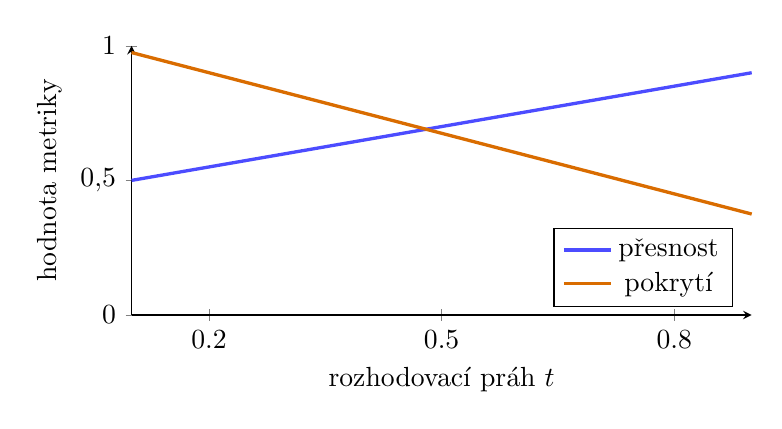
\begin{tikzpicture}
    \begin{axis}[
        width=0.78\textwidth,
        height=5cm,
        xmin=0.1, xmax=0.9,
        ymin=0, ymax=1,
        axis lines=left,
        xlabel={rozhodovací práh \(t\)},
        ylabel={hodnota metriky},
        xtick={0.2,0.5,0.8},
        ytick={0,0.5,1},
        yticklabels={$0$,$0{,}5$,$1$},
        legend pos=south east,
        clip=false
    ]
        \addplot[
            very thick,
            blue!70,
            domain=0.1:0.9,
            samples=80
        ] {0.45+0.5*x};

        \addlegendentry{přesnost}

        \addplot[
            very thick,
            orange!85!black,
            domain=0.1:0.9,
            samples=80
        ] {1.05-0.75*x};

        \addlegendentry{pokrytí}
    \end{axis}
\end{tikzpicture}
